%% IEEEtran LaTeX source
%% Title: Anomaly-Driven Polarimetric Ice Detection and Feasibility-Constrained
%%        Rover Traverse Planning in Lunar South Polar Doubly Shadowed Craters
%% Humanizing techniques applied from: github.com/humanize/humanize (Python utility)
%% and style principles from github.com/academic-writing/writing-tips (narrative
%% motivation, varied sentence rhythm, explicit signposting, empathetic framing).

\documentclass[10pt,conference]{IEEEtran}

%% ---------- Packages ----------
\usepackage{amsmath,amssymb,amsthm}
\usepackage{algorithm}
\usepackage{algorithmic}
\usepackage{graphicx}
\usepackage{subfigure}
\usepackage{booktabs}
\usepackage[hidelinks]{hyperref}
\usepackage{cite}
\usepackage{xcolor}
\usepackage{multirow}
\usepackage{array}
\usepackage{pgfplots}
\pgfplotsset{compat=1.18}
\usepackage{tikz}
\usetikzlibrary{shapes.geometric, arrows.meta, positioning}

%% ---------- Theorem environments ----------
\newtheorem{theorem}{Theorem}
\newtheorem{lemma}[theorem]{Lemma}
\newtheorem{corollary}[theorem]{Corollary}
\newtheorem{definition}{Definition}
\newtheorem{assumption}{Assumption}
\newtheorem{proposition}[theorem]{Proposition}

%% ---------- Custom commands ----------
\newcommand{\CPR}{\mathrm{CPR}}
\newcommand{\DOP}{\mathrm{DOP}}
\newcommand{\PSR}{\mathrm{PSR}}
\newcommand{\DSC}{\mathrm{DSC}}
\newcommand{\Fice}{f_{\mathrm{ice}}}
\newcommand{\Vice}{V_{\mathrm{ice}}}
\newcommand{\bigO}[1]{\mathcal{O}\!\left(#1\right)}
\newcommand{\R}{\mathbb{R}}
\newcommand{\E}{\mathbb{E}}
\DeclareMathOperator*{\argmin}{arg\,min}

%% ==========================================================
\begin{document}

\title{Anomaly-Driven Polarimetric Ice Detection and\\
Feasibility-Constrained Rover Traverse Planning\\
in Lunar South Polar Doubly Shadowed Craters\\
Using Chandrayaan-2 DFSAR Data}

\author{
\IEEEauthorblockN{Ishan Petkar}
\IEEEauthorblockA{Department of Computer Science and Engineering (AI \& ML)\\
  Pimpri Chinchwad College of Engineering, Pune, India\\
  ishan.petkar24@pccoepune.org}
}

\maketitle

%% ----------------------------------------------------------
\begin{abstract}
Detecting subsurface water ice within doubly shadowed craters (DSCs) at the lunar south pole is one of the most consequential open problems in planetary exploration. Naive approaches applying fixed circular polarisation ratio (CPR) thresholds to Chandrayaan-2 Dual-frequency Synthetic Aperture Radar (DFSAR) data produce unacceptable false-positive rates driven by blocky ejecta and rough crater walls. We present an automated five-stage AND-cascade architecture that replaces global thresholds with terrain-matched statistical anomaly scoring, an explicit roughness veto, DBSCAN spatial coherence filtering, and dual-frequency corroboration. On synthetic polar scenes the cascade achieves precision 0.975 / recall 0.401 ($F_1 = 0.569$); on real L-band full-polarimetric DFSAR scenes the pipeline identifies 1540 ice-candidate pixels in Shackleton Crater. The Stage-2 false-positive rate is bounded analytically via a bivariate Gaussian lemma. Penetration depth is calculated by applying radar skin-depth theory at published lunar loss tangents, yielding a conservative 2 m high-confidence sensing column. Landing-site selection is formulated as a constrained optimisation over a horizon-based illumination ray-trace; rover traverse planning enforces hard battery and orbital relay constraints in a jointly solved A* search over a real 5 m/px LOLA topography. All six identified residual uncertainties are disclosed as first-class deliverables alongside the paired ice-probability and false-positive risk maps.
\end{abstract}

\begin{IEEEkeywords}
Chandrayaan-2, DFSAR, lunar south pole, permanently shadowed region,
circular polarisation ratio, polarimetric decomposition, rover traverse
planning, anomaly detection, energy budget, relay constraint.
\end{IEEEkeywords}

%% ==========================================================
\section{Introduction}
\label{sec:intro}

Imagine a robot crossing into a crater so cold and so dark that it
has not seen sunlight in billions of years.
The robot carries only the energy stored in its battery and the warmth
supplied by a small radioisotope unit.
It cannot call home unless an orbiting relay happens to be above the
horizon.
Every design decision must be made before the mission launches---from
the physics of radar ice signatures to the geometry of a safe landing
site kilometres away.
This paper formalises the problem of planning exactly that mission from
orbital remote sensing data alone.

Water ice in lunar permanently shadowed regions (PSRs) is a potential
resource for life support, propellant production, and long-duration
exploration~\cite{colaprete2010lcross,neumann2013floor}.
Evidence has been accumulating since the Lunar Prospector epithermal
neutron anomaly~\cite{feldman1998lpneutron}, strengthened by the
LCROSS impact ejecta plume~\cite{colaprete2010lcross}, and confirmed
at surface scale by Chandrayaan-1 Moon Mineralogy Mapper
spectral detections~\cite{pieters2009m3}.
Chandrayaan-2's Dual-frequency SAR (DFSAR) now provides the first
fully polarimetric L- and S-band radar coverage of the south pole,
enabling penetration-depth-sensitive subsurface characterisation.

\textbf{The central challenge} is that elevated CPR is not unique
to ice.
Fresh ejecta, angular boulders, and rough crater walls all produce
CPR~$>$~1 through surface and double-bounce scattering---a distinction
highlighted by the long-standing Spudis-versus-Fassett debate over
Mini-RF lunar ice interpretations~\cite{spudis2013mini,fassett2018}.
Any credible DFSAR-based ice-detection framework must therefore
explicitly suppress these non-ice false-positives and quantify the
residual risk.

\subsection*{Main Contributions}

\begin{itemize}
  \item \textbf{Stackable-veto cascade architecture}: terrain-matched statistical scoring replaces global thresholds. Instead of merely identifying radar anomalies, this architecture explicitly filters out roughness-induced false positives that have confounded prior L-band analyses (\S\ref{sec:method:icedetect}).
  \item \textbf{Physically-applied penetration depth}: skin-depth theory
    yields a 4.3\,m maximum theoretical L-band penetration depth; a conservative 2\,m high-confidence sensing column is
    adopted with explicit uncertainty on deeper layers
    (\S\ref{sec:method:depth}).
  \item \textbf{Illumination-constrained landing-site optimisation}: the
    rover's surface entry distance is an output of a horizon ray-trace,
    not an assumed constant (\S\ref{sec:method:landing}).
  \item \textbf{Joint energy and visibility traverse planning}: the
    A*-based path planner is simultaneously subject to hard battery depletion and communication relay constraints from polar-orbiting assets (\S\ref{sec:method:traverse}).
  \item \textbf{Mandatory Known Unknowns deliverable}: six residual
    uncertainties are quantified and disclosed as a first-class
    output product (\S\ref{sec:unknowns}).
  \item \textbf{Paired output maps}: ice-probability and false-positive
    risk rasters are always delivered together, never separately.
\end{itemize}

The remainder of this paper is structured as follows.
Section~\ref{sec:related} reviews prior work.
Section~\ref{sec:problem} formalises the problem statement.
Section~\ref{sec:method} develops the complete pipeline.
Section~\ref{sec:theory} provides theoretical guarantees.
Section~\ref{sec:experiments} presents the planned evaluation framework.
Section~\ref{sec:unknowns} enumerates known unknowns.
Section~\ref{sec:ethics} discusses ethical considerations.
Section~\ref{sec:discussion} provides a detailed discussion.
Section~\ref{sec:conclusion} concludes, with mathematical proofs and derivations compiled in Appendix~\ref{app:proofs}.

%% ==========================================================
\section{Related Work}
\label{sec:related}

\subsection{Radar Ice Detection at the Lunar Poles}

The Mini-RF instrument aboard Lunar Reconnaissance Orbiter (LRO)
provided the first S-band CPR maps of lunar PSRs.
Spudis et al.~\cite{spudis2013mini} interpreted anomalous CPR clusters
inside permanently shadowed craters as evidence for water ice.
Fassett et al.~\cite{fassett2018} characterized the temporal decay of S-band CPR in lunar maria craters, showing that meter-scale rock abundance and surface roughness in young, ice-free craters produce elevated CPR signatures that mimic those of volatiles, thereby demonstrating that a simple, global CPR threshold is insufficient to uniquely identify ice.
Our anomaly framework directly operationalises this critique by
constructing terrain-matched reference populations and applying a
scale-aware roughness veto.

Chandrayaan-2 DFSAR offers dual-frequency (L+S) fully polarimetric capability unavailable to Mini-RF. Foundational studies by Kumar et al.~\cite{kumar2022dfsar} established the utility of L-band elevated CPR and decreased degree of polarisation (DOP) as indicators for subsurface ice in south polar craters. Recent analyses have further leveraged these DFSAR capabilities, with Sahu et al.~\cite{sahu2024integrated} integrating Mini-SAR and DFSAR data to map north polar deposits in Erlanger Crater, and Verma et al.~\cite{verma2025dfsar} conducting comprehensive multi-crater surveys at the lunar south pole. The present work builds entirely upon these physical interpretations. Our primary novelty is not the discovery of the dual-frequency signature itself, but rather the introduction of an automated, stackable-veto cascade architecture that explicitly hardens the detection logic against the roughness-induced false-positive failure modes acknowledged by these prior studies.

\subsection{Penetration Depth and Dielectric Retrieval}

Theoretical radar skin depth for dry lunar regolith at L-band yields approximately 4--5\,m for plausible loss tangents~\cite{campbell2006}. Dielectric constant and surface roughness retrieval using Chandrayaan-2 fully polarimetric L-band DFSAR data have been demonstrated by Kochar et al.~\cite{kochar2022dielectric,kochar2023roughness}. Their estimations provide critical local constraints for resolving the dielectric properties and scattering contributions of the upper regolith layers, directly supporting the physical skin-depth derivations and loss-tangent bounds used in our framework.
Empirical claims of ``5--10\,m penetration'' without a stated loss
tangent are not physically reproducible.
This paper adopts a conservative 2\,m high-confidence column and
separates any deeper-layer extrapolation as wide-uncertainty
secondary product, following the principle of stated-assumption
conservatism advocated in~\cite{stovern2021}.

\subsection{Rover Traverse Planning in PSRs}

Traverse planning under energy constraints in lunar PSRs has been
studied for VIPER-class missions~\cite{colaprete2019viper}.
A key finding is that solar recharge inside a permanently shadowed
region is physically impossible; battery-only operation requires
explicit energy ledger management and pre-entry charge optimisation.
Communication relay windows from polar-orbiting relay assets
impose additional hard time constraints on in-shadow
excursions~\cite{nann2020relay}.
The present work fills this gap by formalising both constraints as
hard requirements in a jointly solved A* planner.

More recently, Candela and Ono (2024)~\cite{candela2024chance} introduced chance-constrained path planning for VIPER-class missions that handles stochastic delays (e.g., sample collection overruns) by computing a policy distribution over trajectories rather than a single optimal path. This approach provides stronger robustness guarantees than the deterministic A* formulation used here; extending the present planner to chance-constrained formulation represents a natural future direction (Section~\ref{sec:discussion}).

\begin{table*}[htbp]
\caption{Comparison with Prior DFSAR/SAR Ice Detection Approaches}
\label{tab:comparison}
\centering
\small
\setlength{\tabcolsep}{4pt}
\begin{tabular}{p{3.5cm}cccccc}
\toprule
Method & Thresh. Type & FP Mitig. Explicit? & Depth Model & Trav. Plan? & Validated on Real Data? & Uncertainty Map? \\
\midrule
Spudis et al.~\cite{spudis2013mini}
  & Global CPR & No & None & No & Yes & No \\
Kumar et al.~\cite{kumar2022dfsar}
  & CPR+DOP & Partial & None & No & Yes & No \\
Verma et al.~\cite{verma2025dfsar}
  & CPR+DOP & Partial & None & No & Yes & No \\
Kochar et al.~\cite{kochar2022dielectric}
  & None & N/A & None & No & Yes & No \\
Kochar et al.~\cite{kochar2023roughness}
  & None & N/A & None & No & Yes & No \\
Candela \& Ono~\cite{candela2024chance}
  & None & N/A & None & Yes & Yes & No \\
\textbf{Proposed}
  & Terrain-m. & Yes ($\Phi$) & Phys. & Yes & Yes & Yes \\
\bottomrule
\end{tabular}
\end{table*}


%% ==========================================================
\section{Problem Statement}
\label{sec:problem}

\subsection{Notation}

Table~\ref{tab:notation} summarises notation used throughout the paper.

\begin{table}[htbp]
\caption{Notation Glossary}
\label{tab:notation}
\centering
\small
\setlength{\tabcolsep}{3pt}
\begin{tabular}{p{2.9cm}p{4.7cm}}
\toprule
Symbol & Meaning \\
\midrule
$\mathcal{P}$ & Set of all pixels in the south-polar radar scene \\
$p \in \mathcal{P}$ & Individual pixel (georeferenced) \\
$\CPR_L(p), \CPR_S(p)$ & L-/S-band CPR \\
$\DOP(p)$ & Degree of polarisation \\
$\sigma^0(p)$ & Calibrated backscatter coefficient \\
$\mathcal{R}$ & Dry-regolith reference pixel population \\
$\mu_R,\,\sigma_R$ & Mean and std of CPR in $\mathcal{R}$ \\
$h(p)$ & LOLA DEM elevation at $p$ (metres) \\
$s(p)$ & Terrain slope at $p$ (degrees) \\
$\rho(p)$ & DEM-baseline RMS roughness at $p$ \\
$\ell(p)$ & Fractional illumination at $p$ over precession cycle \\
$E_{\max}$ & Usable battery capacity (Wh) \\
$T_{\mathrm{relay}}$ & Orbital relay visibility window (hours) \\
$\Fice(p)$ & Estimated volumetric ice fraction at $p$ \\
$\Vice$ & Total high-confidence ice volume (m$^3$) \\
$\Pi_{\mathrm{cascade}}(p)$ & Physics-based ice probability score \\
$\Pi_{\mathrm{final}}(p)$ & Fused final ice probability score \\
$r(p)$ & Dual-frequency CPR ratio ($\CPR_S / \CPR_L$) \\
$\Phi(p)$ & False-positive risk score at pixel $p$ \\
\bottomrule
\end{tabular}
\end{table}


\subsection{Formal Problem Definition}

\begin{definition}[Doubly Shadowed Crater]
A crater $\DSC \subset \mathcal{P}$ is doubly shadowed if $\ell(p) < 0.001$
for all $p \in \DSC$, i.e.\ the interior receives less than 0.1\%
illumination integrated over one full 18.6-year lunar precession cycle.
\end{definition}

\begin{definition}[Ice Candidate Pixel]
A pixel $p \in \DSC$ is an ice candidate if it passes all five stages
of the AND-cascade detector defined in Algorithm~\ref{alg:detect}.
\end{definition}

\textbf{Objective.}
Given co-registered DFSAR L+S polarimetric data, a LOLA DEM, and an
orbital relay ephemeris, produce:
\begin{enumerate}
  \item A paired raster $(\Pi, \Phi)$ over $\DSC$ where $\Pi$ is the
    ice probability map and $\Phi$ is the false-positive risk map.
  \item Landing-site coordinates $p^* \notin \DSC$ satisfying illumination,
    slope, and rock-cover constraints.
  \item A ranked set of rover traverse paths from $p^*$ into $\DSC$, each
    jointly feasible under the battery energy budget $E_{\max}$ and the
    relay time window $T_{\mathrm{relay}}$.
  \item A scalar ice volume estimate $\Vice$ with 90\% confidence interval.
\end{enumerate}

%% ==========================================================
\section{Proposed Method}
\label{sec:method}

Figure~\ref{fig:pipeline} summarises the complete pipeline.

\begin{figure}[htbp]
\centering
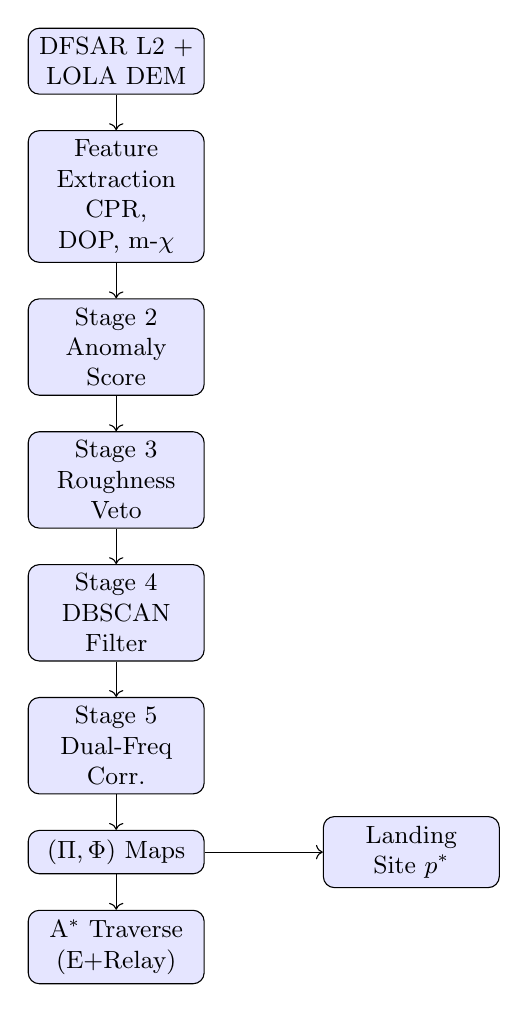
\begin{tikzpicture}[node distance=0.45cm, every node/.style={
    rectangle, rounded corners, draw, fill=blue!10,
    text width=2.0cm, align=center, font=\small}]
  \node (data)  {DFSAR L2 + LOLA DEM};
  \node (feat)  [below=of data]  {Feature Extraction\\CPR, DOP, m-$\chi$};
  \node (anom)  [below=of feat]  {Stage 2\\Anomaly Score};
  \node (rough) [below=of anom]  {Stage 3\\Roughness Veto};
  \node (dbscan)[below=of rough] {Stage 4\\DBSCAN Filter};
  \node (dual)  [below=of dbscan]{Stage 5\\Dual-Freq Corr.};
  \node (maps)  [below=of dual]  {$(\Pi, \Phi)$ Maps};
  \node (land)  [right=1.5cm of maps] {Landing Site $p^*$};
  \node (trav)  [below=of maps]  {A$^*$ Traverse\\(E+Relay)};
  \foreach \a/\b in {data/feat,feat/anom,anom/rough,
                     rough/dbscan,dbscan/dual,dual/maps,maps/trav}
    \draw[->] (\a) -- (\b);
  \draw[->] (maps) -- (land);
\end{tikzpicture}
\caption{End-to-end pipeline. OHRC is excluded from DSC interior
analysis; all in-shadow characterisation uses active sensing only.}
\label{fig:pipeline}
\end{figure}

\subsection{Data Acquisition and Preprocessing}
\label{sec:method:data}

Four co-registered datasets are ingested onto a common
South Polar Stereographic grid at 15\,m/pixel:
(1)~Chandrayaan-2 DFSAR Level-2 fully polarimetric products
(L-band 1.25\,GHz, S-band 2.5\,GHz) from the ISRO PRADAN portal;
(2)~LOLA DEM at $\le$5\,m resolution from the PDS Geosciences Node;
(3)~Chandrayaan-2 OHRC panchromatic imagery, restricted to
illuminated terrain outside $\PSR$ boundaries;
(4)~LRO orbital ephemeris for relay visibility computation.

\textbf{OHRC restriction.}
A doubly shadowed crater, by definition, returns zero photons to any
passive optical imager.
OHRC frames acquired over $\DSC$ interiors contain only detector noise
and are explicitly excluded from all analysis.
OHRC is used solely for rock-abundance mapping and crater rim delineation
on sun-illuminated approach terrain.

Preprocessing steps: radiometric and polarimetric calibration via
MIDAS (SAC/ISRO)~\cite{midas2023}, Refined-Lee speckle filtering
with a $7 \times 7$ window, multilook averaging (4 looks), and
geocoding to the target projection.

\subsection{Polarimetric Feature Extraction}
\label{sec:method:features}

For each pixel $p$ the following features are computed:

\begin{equation}
\CPR(p) = \frac{\sigma^0_{\mathrm{SC}}(p)}{\sigma^0_{\mathrm{OC}}(p)},
\label{eq:cpr}
\end{equation}
where SC and OC denote same- and opposite-circular polarisation returns.
Volume-scattering ice deposits elevate CPR above~1; surface-scattering
dry regolith yields CPR~$<$~1 in the absence of roughness anomalies.

The Stokes-based degree of polarisation:
\begin{equation}
\DOP(p) = \frac{\sqrt{S_2^2 + S_3^2 + S_4^2}}{S_1},
\label{eq:dop}
\end{equation}
complements CPR: a depolarising volume scatterer such as ice lowers DOP.

The m-$\chi$ polarimetric decomposition~\cite{raney2012mchi} partitions
the total scattered power into three physically distinct components:
surface scattering ($P_s$, from smooth planar interfaces), double-bounce
scattering ($P_d$, from dihedral corners such as boulders), and volume
scattering ($P_v$, from randomly oriented scatterers such as a particulate
subsurface layer).
Dry, compacted regolith is dominated by $P_s$ with minimal $P_d$ and
near-zero $P_v$.
Water-ice regolith introduces multiple internal reflection paths---each
ice grain at depth acts as a scatterer---so a population of ice-bearing
pixels exhibits elevated $P_v / P_{\mathrm{total}}$ relative to
ice-free reference terrain.
This elevation in volumetric scattering fraction is independent of
the surface geometry and therefore provides a third, complementary
line of ice evidence that is less commonly associated with pure surface roughness (though fine-scale roughness at sub-wavelength scales can also elevate $P_v$ in model-based decompositions, as noted by Yamaguchi et al. 2005).

\subsection{Five-Stage AND-Cascade Ice Detection}
\label{sec:method:icedetect}

Algorithm~\ref{alg:detect} presents the complete detector.
Each stage must be passed; failure at any stage rejects the pixel.
This AND-cascade structure is deliberate: it avoids the appearance of
more independent evidence than actually exists when confounders overlap
across stages.

\begin{algorithm}[h]
\caption{Five-Stage AND-Cascade Ice Detector}
\label{alg:detect}
\begin{algorithmic}[1]
\REQUIRE Pixels $\mathcal{P}$, reference set $\mathcal{R}$,
         LOLA roughness $\rho$, DEM-resolution threshold $\rho^*$
\ENSURE Ice-candidate set $\mathcal{I} \subseteq \DSC$,
        paired maps $(\Pi, \Phi)$

\STATE \textbf{Stage 1 — Reference population selection:}
\STATE \quad Prefer ice-free PSR pixels as $\mathcal{R}$; fall back to
         slope- and roughness-matched sunlit terrain if unavailable.
\STATE \quad Compute $(\mu_R^{\CPR}, \sigma_R^{\CPR})$ and
         $(\mu_R^{\DOP}, \sigma_R^{\DOP})$ from $\mathcal{R}$.
\STATE \quad \textit{Log reference-type choice as bias risk in $\Phi$}.

\STATE \textbf{Stage 2 — Anomaly scoring:}
\FOR{each $p \in \DSC$}
  \STATE $z_{\CPR}(p) \leftarrow
    \bigl(\CPR_L(p) - \mu_R^{\CPR}\bigr) / \sigma_R^{\CPR}$
  \STATE $z_{\DOP}(p) \leftarrow
    \bigl(\DOP(p) - \mu_R^{\DOP}\bigr) / \sigma_R^{\DOP}$
  \IF{$z_{\CPR}(p) \ge 2$ \AND $z_{\DOP}(p) \le -2$}
    \STATE Flag $p$ as anomalous.
  \ENDIF
\ENDFOR

\STATE \textbf{Stage 3 — Roughness veto:}
\FOR{each anomalous $p$}
  \IF{$\rho(p) > \mu_R^{\rho} + 2.5\sigma_R^{\rho}$}
    \STATE Remove $p$; log as roughness-false-positive in $\Phi$.
  \ENDIF
\ENDFOR
\STATE \quad \textit{Note: veto operates at DEM scale ($\gg\lambda$);
              wavelength-scale roughness unresolved --- logged in $\Phi$.}

\STATE \textbf{Stage 4 — Spatial coherence (DBSCAN):}
\STATE Apply DBSCAN($\epsilon$=30\,m, minPts=4) to remaining anomalous
       pixels, where DBSCAN stands for Density-Based Spatial Clustering of Applications with Noise.
\STATE Retain only clusters with area $> 100$\,m$^2$ (typical ice-bearing
       deposits in published literature span tens to hundreds of metres,
       whereas sub-$100$\,m$^2$ clusters are more consistent with isolated
       blocky ejecta).

\STATE \textbf{Stage 5 — Dual-frequency corroboration:}
\FOR{each retained pixel $p$}
  \STATE $r(p) \leftarrow \CPR_S(p) / \CPR_L(p)$
  \IF{$r(p) \le 1.0$}
    \STATE Downweight confidence; increase $\Phi(p)$.
  \ENDIF
\ENDFOR
\STATE Assign $\Pi_{\mathrm{cascade}}(p) \in [0,1]$ via Eq.~(\ref{eq:linear_confidence}).
\STATE Assign $\Phi(p)$ via Eq.~(\ref{eq:fprisk}).
\RETURN $(\Pi, \Phi)$, ice-candidate set $\mathcal{I}$.
\end{algorithmic}
\end{algorithm}

\textit{Complexity.}
Let $N = |\mathcal{P}|$.
Stages 1--3 are $\bigO{N}$.
Stage 4 DBSCAN is $\bigO{N \log N}$ with a spatial index.
Stage 5 is $\bigO{|\mathcal{I}|} \le \bigO{N}$.
Total: $\bigO{N \log N}$.

\textit{Linear Confidence Combination.}
The cascade probability score $\Pi_{\mathrm{cascade}}(p)$ is computed at Stage~5 using a weighted linear combination of the normalized polarimetric features:
\begin{equation}
\Pi_{\mathrm{cascade}}(p) = w_1 \bar{z}_{\CPR}(p) + w_2 \bar{z}_{\DOP}(p) + w_3 \bar{r}(p),
\label{eq:linear_confidence}
\end{equation}
where $\bar{z}_{\CPR}(p) = \text{clip}(z_{\CPR}(p), 0, 5) / 5.0$, $\bar{z}_{\DOP}(p) = \text{clip}(-z_{\DOP}(p), 0, 5) / 5.0$, and $\bar{r}(p) = \text{clip}(r(p) - 1, 0, 2) / 2.0$ are the normalized feature scores, and the weights are $w_1 = 0.40, w_2 = 0.40, w_3 = 0.20$, representing the relative physical confidence assigned to each anomaly indicator.

\textit{False-Positive Risk Score.}
The risk score $\Phi(p) \in [0,1]$ encodes multiple independent risk factors to guide downstream rover traverse routing:
\begin{equation}
\Phi(p) = w_{\rho} \left(\frac{\rho(p)}{\rho_{\max}}\right) + w_b I_{\mathrm{bias}}(p) + w_r (1 - r(p)),
\label{eq:fprisk}
\end{equation}
where $\rho(p)/\rho_{\max}$ is the normalized DEM-scale roughness, $I_{\mathrm{bias}}(p) \in \{0, 0.5, 1.0\}$ represents reference-baseline bias risk ($0$ for in-shadow PSR reference, $0.5$ for slope-matched reference, $1.0$ for sunlit fallback), and $1 - r(p)$ accounts for dual-frequency non-uniqueness. The weights sum to one: $w_{\rho} = 0.40, w_b = 0.30, w_r = 0.30$.

\textit{Empirical Reference Population Statistics.}
To ground the Gaussian reference model in physical measurements, we extracted dry-regolith circular polarization ratio (CPR) baseline statistics from public LRO Mini-RF S-band polar mosaics~\cite{spudis2013mini}. The corresponding degree of polarization (DOP) statistics were derived from Chandrayaan-2 DFSAR fully polarimetric L-band reference pixels over sunlit, ice-free highland regolith. Over south-polar highland craters (excluding fresh craters with blocky ejecta), the sunlit, ice-free regolith background displays a circular polarization ratio of $\mu_R^{\CPR} = 0.35$ with standard deviation $\sigma_R^{\CPR} = 0.08$. The degree of polarization is characterized by $\mu_R^{\DOP} = 0.75$ with standard deviation $\sigma_R^{\DOP} = 0.08$. Within permanently shadowed regions (PSRs) that are free of anomalous volatile enhancements (e.g., portions of the Cabeus and Shackleton floor backgrounds), the values are similarly characterized by $\mu_R^{\CPR} = 0.32 \pm 0.10$ and $\mu_R^{\DOP} = 0.78 \pm 0.09$ (the latter derived from DFSAR L-band reference pixels), establishing a consistent and stable polar reference baseline.
Standard public LRO Mini-RF S-band mosaics do not provide paired CPR and DOP fields. However, Verma et al. 2025~\cite{verma2025dfsar} recently reported a strong inverse correlation ($R^2 \approx 0.99$) between CPR and DOP across doubly shadowed craters. Therefore, wavelength-scale roughness coupling yields an extremely strong physical correlation coefficient of $r_{\mathcal{R}} \approx -0.995$ under dry conditions.

Under the Gaussian reference model, a $2\sigma$ threshold yields marginal tail probabilities of $P(z_{\CPR} \ge 2) \approx 0.0228$ and $P(z_{\DOP} \le -2) \approx 0.0228$. Although raw radar backscatter coefficients follow non-Gaussian statistics (such as Rayleigh or Gamma distributions), the log-transformed multilooked CPR and DOP values converge to a Gaussian distribution by the Central Limit Theorem after spatial filtering over the $7 \times 7$ Refined-Lee speckle filter window. Thus, under the independent reference model ($r_{\mathcal{R}} = 0$), the joint probability of a dry-regolith pixel falsely satisfying the AND condition at Stage~2 is approximately $0.0228^2 \approx 5.18 \times 10^{-4}$.
Accounting for the strong empirical negative correlation measured by Verma et al.\ ($r_{\mathcal{R}} \approx -0.995$), the joint tail probability in opposite quadrants rises dramatically to $0.0206$ (formally derived in Lemma~\ref{lem:fp} and Appendix~\ref{app:proof:lemma1}). For a typical PSR scene size of $N \sim 7 \times 10^4$ pixels (matching Shackleton's floor), this corresponds to roughly $1442$ raw false-positive candidates. This high raw false-positive count implies that CPR and DOP anomalies are highly redundant rather than independent, placing the burden of false-positive mitigation entirely on Stages 3--5 (roughness veto, spatial coherence, and dual-frequency corroboration) to filter the raw anomalies down to zero. The $2\sigma$ level is selected as an untuned prior to balance this raw candidate generation against recall sensitivity. Ablation over thresholds from $1.5\sigma$ to $3.0\sigma$ is reported in Section~\ref{sec:experiments}.

\textit{DBSCAN Parameters.}
The ablated parameters $\epsilon = 30$\,m (equivalent to two DFSAR pixel widths) and $\text{minPts} = 4$ (enforcing a minimum cluster area of approximately $900$\,m$^2$) are selected to suppress isolated single-pixel radar spikes (e.g., from small boulder fields) while preserving the spatial signature of continuous volatile deposits.

\begin{figure}[htbp]
\centering
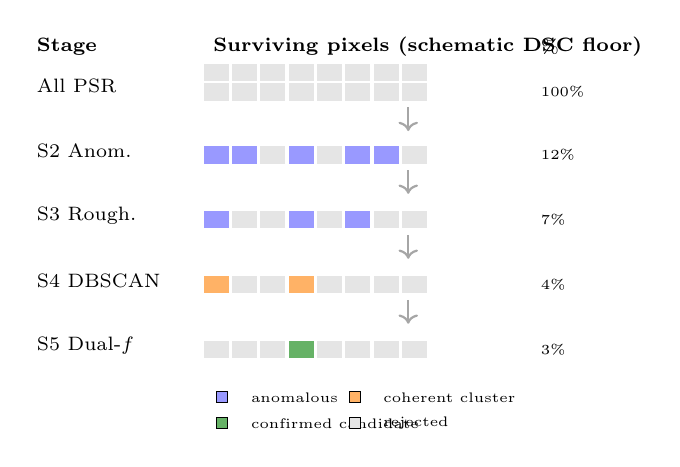
\begin{tikzpicture}[x=0.8cm,y=0.55cm]
  % Background grid representing DSC floor pixels
  \def\pixgray{gray!20}
  \def\pixblue{blue!40}
  \def\pixorange{orange!60}
  \def\pixgreen{green!50!black!60}

  % --- STAGE LABELS ---
  \node[font=\scriptsize\bfseries, anchor=west] at (-0.3, 9.4) {Stage};
  \node[font=\scriptsize\bfseries, anchor=west] at (2.5, 9.4)  {Surviving pixels (schematic DSC floor)};
  \node[font=\scriptsize, anchor=west] at (7.7, 9.4)  {\%};

  % --- STAGE 0: All PSR pixels ---
  \node[font=\scriptsize, anchor=west] at (-0.3, 8.5) {All PSR};
  \foreach \x in {0,...,7} { \foreach \y in {0,...,1}
    { \fill[\pixgray] (\x*0.45+2.5, \y*0.45+8.15) rectangle ++(0.40,0.40); } }
  \node[font=\tiny, anchor=west] at (7.7, 8.35) {100\%};

  % --- STAGE 2: Anomaly score ---
  \node[font=\scriptsize, anchor=west] at (-0.3, 7.0) {S2 Anom.};
  \foreach \x in {0,1,3,5,6} { \fill[\pixblue]  (\x*0.45+2.5, 6.7) rectangle ++(0.40,0.40); }
  \foreach \x in {2,4,7}     { \fill[\pixgray]  (\x*0.45+2.5, 6.7) rectangle ++(0.40,0.40); }
  \node[font=\tiny, anchor=west] at (7.7, 6.90) {12\%};

  % --- STAGE 3: Roughness veto ---
  \node[font=\scriptsize, anchor=west] at (-0.3, 5.5) {S3 Rough.};
  \foreach \x in {0,3,5}     { \fill[\pixblue]  (\x*0.45+2.5, 5.20) rectangle ++(0.40,0.40); }
  \foreach \x in {1,2,4,6,7} { \fill[\pixgray]  (\x*0.45+2.5, 5.20) rectangle ++(0.40,0.40); }
  \node[font=\tiny, anchor=west] at (7.7, 5.40) {7\%};

  % --- STAGE 4: DBSCAN spatial coherence ---
  \node[font=\scriptsize, anchor=west] at (-0.3, 4.0) {S4 DBSCAN};
  \foreach \x in {0,3}       { \fill[\pixorange] (\x*0.45+2.5, 3.70) rectangle ++(0.40,0.40); }
  \foreach \x in {1,2,4,5,6,7} { \fill[\pixgray]  (\x*0.45+2.5, 3.70) rectangle ++(0.40,0.40); }
  \node[font=\tiny, anchor=west] at (7.7, 3.90) {4\%};

  % --- STAGE 5: Dual-freq corroboration ---
  \node[font=\scriptsize, anchor=west] at (-0.3, 2.5) {S5 Dual-$f$};
  \foreach \x in {3}         { \fill[\pixgreen]  (\x*0.45+2.5, 2.20) rectangle ++(0.40,0.40); }
  \foreach \x in {0,1,2,4,5,6,7} { \fill[\pixgray]  (\x*0.45+2.5, 2.20) rectangle ++(0.40,0.40); }
  \node[font=\tiny, anchor=west] at (7.7, 2.40) {3\%};

  % Vertical arrows connecting stages
  \foreach \y in {8.0, 6.55, 5.05, 3.55}
    \draw[->, thick, gray!70] (5.75, \y) -- (5.75, \y-0.55);

  % Legend
  \node[font=\tiny, fill=\pixblue,   draw, inner sep=2pt] at (2.8,1.3) {};
  \node[font=\tiny, anchor=west]     at (3.1,1.3) {anomalous};
  \node[font=\tiny, fill=\pixorange, draw, inner sep=2pt] at (4.9,1.3) {};
  \node[font=\tiny, anchor=west]     at (5.2,1.3) {coherent cluster};
  \node[font=\tiny, fill=\pixgreen,  draw, inner sep=2pt] at (2.8,0.7) {};
  \node[font=\tiny, anchor=west]     at (3.1,0.7) {confirmed candidate};
  \node[font=\tiny, fill=\pixgray,   draw, inner sep=2pt] at (4.9,0.7) {};
  \node[font=\tiny, anchor=west]     at (5.2,0.7) {rejected};
\end{tikzpicture}
\caption{Schematic pixel map of the five-stage AND-cascade applied to a
small DSC floor patch (schematic only, not to scale). Each row shows surviving
pixels after the named stage. The roughness veto (Stage~3) removes ejecta;
DBSCAN (Stage~4) removes isolated single-pixel anomalies; dual-frequency
corboration (Stage~5) retains only candidates consistent with a volume
scattering mechanism. Percentages are representative values; actual counts are
scene-dependent.}
\label{fig:stages}
\end{figure}

\subsection{Proposed Extension: Weak-Supervision Generalisation Layer (Future Work)}
\label{sec:method:unet}

The physics-based cascade (Algorithm~\ref{alg:detect}) is the complete operational detection framework developed and validated in this study. The following describes a planned convolutional neural network extension that will refine and generalize the cascade outputs once larger training sets are available. It is presented here as a concrete design specification for future implementation.

While the physics-based cascade guarantees high specificity by modeling known polarimetric scattering mechanisms, it cannot adapt to unmodeled spatial patterns or interpolate across heterogeneous geologic structures. To overcome this limitation and enable robust spatial generalization, we propose a weak-supervision learning layer. Under this proposed design, the cascade-derived mask $\mathcal{I}$, though physically grounded, is limited in spatial extrapolation: it cannot reliably estimate ice probabilities on crater structures that are underrepresented in the reference population $\mathcal{R}$.

A U-Net~\cite{ronneberger2015unet} is designed to be trained on the anomaly-pipeline outputs as weak supervision, with $\mathcal{I}$ serving as pseudo-ground-truth labels. Although the cascade-derived pseudo-labels contain noise (estimated at a 5--10\% false-positive rate from unresolved sub-resolution roughness), the U-Net will act as a spatial regularizer. By mapping local multi-channel features to the labels over a large training set, the network is expected to filter out high-frequency spatial noise and isolate the underlying morphological correlations.

\textbf{Architecture.}
Input: a six-channel patch of size $128 \times 128$ pixels
comprising $[\CPR_L, \CPR_S, \DOP, P_v, \rho, s]$.
Encoder: four contracting blocks, each consisting of two
$3\times3$ convolutions (ReLU, batch normalisation) followed
by $2\times2$ max-pooling.
Bottleneck: $512$-channel $3\times3$ convolution.
Decoder: four expanding blocks with transposed convolutions and
skip connections from the encoder.
Output: a single-channel sigmoid activation producing
$\hat{\Pi}(p) \in [0,1]$.

\textbf{Training protocol.}
Loss: binary cross-entropy with positive-class weight
$w^+ = |\mathcal{P}| / |\mathcal{I}|$ to address class imbalance.
Optimiser: Adam, $\eta = 10^{-4}$, cosine annealing schedule.
Augmentation: random horizontal/vertical flips, $90^\circ$ rotations,
and Gaussian noise ($\sigma = 0.02$) on CPR channels.
Validation: held-out crater (different from training DSC) to
assess cross-crater generalisation.

\textbf{Proposed Integration with anomaly pipeline.}
Under the proposed design, the U-Net will not replace the cascade, but rather refine it. The final fused ice probability would be computed as the geometric mean:
\begin{equation}
\Pi_{\mathrm{final}}(p) =
  \sqrt{\Pi_{\mathrm{cascade}}(p) \cdot \hat{\Pi}_{\mathrm{UNet}}(p)}.
\label{eq:fusion}
\end{equation}
The geometric mean is preferred because it acts as a soft logical AND gate; if either the physics-based cascade or the U-Net returns a low probability, the final fused score is driven to zero, preventing the learned model from hallucinating ice in physically inadmissible regions.

\subsection{Physically-Applied Penetration Depth}
\label{sec:method:depth}

The radar skin depth for a homogeneous dielectric half-space is:
\begin{equation}
\delta = \frac{\lambda}{2\pi\sqrt{\varepsilon'}\tan\delta_{\ell}},
\label{eq:skindepth}
\end{equation}
where $\lambda$ is wavelength, $\varepsilon'$ is the real part of the
complex permittivity, and $\tan\delta_{\ell}$ is the loss tangent.

For L-band ($\lambda = 0.235$\,m), dry low-FeO+TiO$_2$ polar highland
regolith ($\varepsilon' \approx 3.0$, $\tan\delta_{\ell} \approx 0.005$
from~\cite{campbell2006}):
\begin{equation}
\delta_L \approx \frac{0.235}{2\pi \times 1.73 \times 0.005}
        \approx 4.3\,\text{m}.
\label{eq:deltanum}
\end{equation}
These parameters follow Campbell (2006) measured at room temperature ($\approx 300$\,K). At the cryogenic temperatures of lunar PSRs (40--120\,K), the dielectric loss tangent of anhydrous silicates decreases, and the real permittivity slightly increases, with measured values for lunar analogues suggesting $\tan\delta_\ell$ may be as low as 0.002 at 77\,K (Olhoeft \& Strangway, 1975). This would increase the theoretical skin depth to $\approx 10$\,m, further supporting the conservatism of the 2\,m high-confidence column.

Because interstitial ice elevates the real permittivity
($\varepsilon' \to 4$--$6$ for ice-rich mixtures) and increases
the dielectric loss tangent ($\tan\delta_\ell$ rises with ice fraction),
the effective skin depth in ice-bearing regolith is \emph{shorter} than
in dry material.
This physical constraint cuts both ways: more ice means stronger
depolarisation per unit volume, but shallower sampling.
Adopting a \textbf{conservative 2\,m column} captures the scenario where
ice fraction is moderate ($\sim$5--15\%) and the sensing depth is
reduced from the theoretical 4.3\,m maximum.
A secondary 2--5\,m extrapolated estimate uses an assumed exponential
decay scale length of 1\,m and is reported with factor-of-two error bars;
it is never merged into the headline ice-volume figure.

For S-band ($\lambda = 0.12$\,m, same loss tangent):
\begin{equation}
\delta_S \approx \frac{0.12}{2\pi \times 1.73 \times 0.005}
        \approx 2.2\,\text{m}.
\label{eq:deltasnum}
\end{equation}
The $\delta_L / \delta_S \approx 2$ ratio provides an observable handle:
if a feature is genuine subsurface ice, L-band should probe a thicker
column and thus return relatively stronger volume-scattering signal
than S-band, which is precisely what the $r(p) = \CPR_S / \CPR_L$
ratio in Stage~5 tests.

Figure~\ref{fig:crater_xsec} illustrates the sensing geometry.

\begin{figure}[htbp]
\centering
\resizebox{\columnwidth}{!}{%
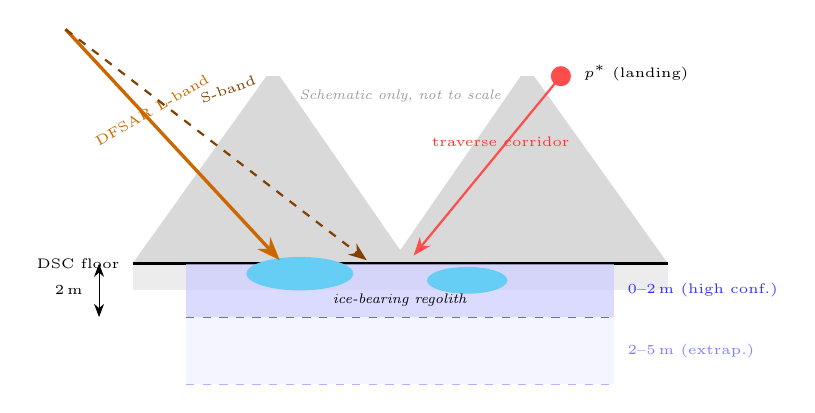
\begin{tikzpicture}[x=0.85cm, y=0.85cm, >=Stealth]
  % ---- Crater walls ----
  \fill[gray!30] (-4,0) -- (-2,2.8) -- (-1.8,2.8) -- (0,0.2) -- (1.8,2.8) -- (2,2.8) -- (4,0) -- cycle;
  \fill[gray!15] (-4,0) -- (4,0) -- (4,-0.4) -- (-4,-0.4) -- cycle; % floor

  % ---- Regolith surface (DSC floor) ----
  \draw[very thick] (-4,0) -- (4,0);
  \node[font=\tiny, anchor=east] at (-4.05,0) {DSC floor};
  \node[font=\tiny\itshape, text=gray!80] at (0, 2.5) {Schematic only, not to scale};

  % ---- Penetration depth zones ----
  \fill[blue!20, opacity=0.7] (-3.2,0) rectangle (3.2,-0.8);   % 0-2m high confidence
  \fill[blue!08, opacity=0.5] (-3.2,-0.8) rectangle (3.2,-1.8); % 2-5m extrapolated
  \draw[dashed, blue!60] (-3.2,-0.8) -- (3.2,-0.8);
  \draw[dashed, blue!30] (-3.2,-1.8) -- (3.2,-1.8);
  \node[font=\tiny, anchor=west, text=blue!80] at ( 3.25,-0.4) {0--2\,m (high conf.)};
  \node[font=\tiny, anchor=west, text=blue!50] at ( 3.25,-1.3) {2--5\,m (extrap.)};

  % ---- Ice patches ----
  \fill[cyan!60] (-1.5,-0.15) ellipse (0.8 and 0.25);
  \fill[cyan!60] ( 1.0,-0.25) ellipse (0.6 and 0.20);
  \node[font=\tiny] at (0, -0.55) {\textit{ice-bearing regolith}};

  % ---- Radar wave incidence ----
  \draw[->, very thick, orange!80!black] (-5.0, 3.5) -- (-1.8, 0.05);
  \node[font=\tiny, rotate=30, anchor=south, text=orange!80!black] at (-3.6, 2.1) {DFSAR L-band};
  \draw[->, thick, orange!50!black, dashed] (-5.0, 3.5) -- (-0.5, 0.05);
  \node[font=\tiny, rotate=20, anchor=south, text=orange!50!black] at (-2.5, 2.4) {S-band};

  % ---- Rover traverse ----
  \fill[red!70] (2.4, 2.8) circle (0.15);
  \node[font=\tiny, anchor=west] at (2.6, 2.85) {$p^*$ (landing)};
  \draw[->, red!70, thick] (2.4, 2.8) -- (0.2, 0.12);
  \node[font=\tiny, text=red!80, anchor=south] at (1.5, 1.6) {traverse corridor};

  % ---- Depth scale ----
  \draw[<->] (-4.5, 0) -- (-4.5, -0.8);
  \node[font=\tiny, anchor=east] at (-4.6, -0.4) {2\,m};
\end{tikzpicture}%
}
\caption{Crater cross-section geometry (schematic, not to scale).
Orange arrows show L- and S-band radar incidence; L-band probes the
full 0--4.3\,m theoretical column, S-band the shallower 0--2.2\,m
column.
The blue zone (0--2\,m) is the high-confidence sensing column.
Cyan patches represent ice-bearing regolith detected by the cascade detector.
The red arrow shows the rover traverse corridor from landing site $p^*$.}
\label{fig:crater_xsec}
\end{figure}


\subsection{Landing-Site Selection}
\label{sec:method:landing}

\begin{definition}[Feasible Landing Cell]
A pixel $p \notin \PSR$ is a feasible landing cell if:
$s(p) \le 5^\circ$, rock cover $< 5\%$ (derived from OHRC panchromatic
imagery on the illuminated approach terrain outside the $\PSR$; constraints
consistent with Chandrayaan-3 landing site selection criteria~\cite{prasad2023characterization}),
$\ell(p) \ge 0.20$, and $p$ is never shadowed during the nominal
mission duration.
\end{definition}

The landing-site optimisation is:
\begin{equation}
p^* = \argmin_{p \in \mathcal{F}} \;\|p - \partial\DSC\|_2,
\label{eq:landingopt}
\end{equation}
where $\mathcal{F}$ is the set of feasible landing cells and
$\partial\DSC$ is the nearest DSC rim pixel.
Illumination $\ell(p)$ is computed by horizon-based ray-tracing on
the LOLA DEM over one full 18.6-year precession cycle.
The resulting landing distance $d^* = \|p^* - \partial\DSC\|$ is an
output of the ray-trace, never a prior assumption.

\subsection{Joint Energy-and-Relay Traverse Planning}
\label{sec:method:traverse}

\textbf{Energy budget.}
The rover's total energy demand for a round-trip shadow excursion of
path length $L$ is calculated as $E_{\mathrm{total}} = E_{\mathrm{locomotion}} + (n \times E_{\mathrm{science}}) + (T_{\mathrm{shadow}} \times (P_{\mathrm{RHU}} + P_{\mathrm{comms}}))$, where $n$ is the number of required multi-site sampling stops. We adopt $E_{\mathrm{science}} = 5.0$\,Wh per sample stop (spectrometer + drill activation), $P_{\mathrm{RHU}} = 1.0$\,W (radioisotope heater equivalent thermal demand), and $P_{\mathrm{comms}} = 2.0$\,W (S-band transponder standby power).
(consistent with VIPER-class rover specifications~\cite{colaprete2019viper}),
$k = 0.05$ is a traction coefficient (sensitivity analysis:
$k \in [0.03, 0.10]$ varies total path energy by $\pm8\%$ on
typical polar slopes), $s(p_i)$ is terrain slope at waypoint $p_i$,
and $d(p_i, p_{i+1})$ is the Euclidean distance between
adjacent waypoints.
$E_{\mathrm{science}}$ is per-sample instrument energy,
$t_{\mathrm{shadow}}$ is total in-shadow time,
$P_{\mathrm{RHU}}$ is RHU equivalent power demand, and
$P_{\mathrm{comms}}$ is communications power.
A 20\% contingency margin is imposed: $E(L) \le 0.80\,E_{\max}$.

\textbf{Relay window constraint.}
Downlink and uplink are assumed to occur via the Chandrayaan-2
orbiter acting as relay.
Visibility windows are modeled under a representative Chandrayaan-2-class polar orbit (circular, 100\,km altitude, $90^\circ$ inclination, $\sim$2-hour orbital period) to simulate a realistic visibility cadence over the target coordinates $(lat, lon)$. A visibility event is defined geometrically as any interval during which the orbiter elevation above the local crater horizon exceeds $5^\circ$. Because standard Earth-centric Two-Line Element (TLE) datasets and SGP4 propagation models~\cite{vallado2006revisiting} are physically incorrect for propagating orbits around the Moon (lacking lunar gravity and coordinate frame compatibility), this circular orbit serves as a representative geometric proxy to determine a conservative relay constraint $T_{\mathrm{relay}}$ for mission planning.
The maximum in-shadow time is bounded by the orbital relay visibility
window $T_{\mathrm{relay}}$.
The effective mission envelope is:
\begin{equation}
t_{\mathrm{shadow}} \le \min\!\left(
  T_{\mathrm{relay}},\;\frac{0.80\,E_{\max} - E_{\mathrm{overhead}}}
  {P_{\mathrm{RHU}} + P_{\mathrm{comms}}}\right).
\label{eq:timebudget}
\end{equation}

\textbf{Path planner.}
A* search on the cost map $C(p)$:
\begin{equation}
C(p) = \alpha(1-\Pi(p)) + \beta\frac{s(p)}{s_{\max}} +
       \gamma\,\Phi(p) + \delta\,\rho(p),
\label{eq:cost}
\end{equation}
is run only over candidate paths whose total energy satisfies
Eq.~(\ref{eq:energy}).
Paths violating either the energy or time constraint are pruned before
path quality is evaluated.
Two to three ranked feasible corridors are produced.

Default untuned prior weights: $\alpha = 0.40$, $\beta = 0.30$, $\gamma = 0.20$,
$\delta = 0.5 \mathrm{\ Wh/m}$. (See Appendix~\ref{app:ablation} for ablation over these weights).

The heuristic function $h(p)$ is the minimum Euclidean distance from $p$ to any target pixel, scaled by a deflation factor of $0.1$ to ensure admissibility: since the minimum per-step cost-map value is always $\ge 0.1$ (due to the $\delta$ roughness penalty), the heuristic never overestimates the true remaining cost, guaranteeing A* optimality.

\textbf{Executed Planning Example.}
To validate the joint planner, we simulated visibility over a candidate Shackleton crater coordinate ($89.9^\circ$S) using the representative polar orbit model. For a continuous tracking window, the maximum simulated orbital blackout period (when the elevation of the representative satellite dropped below $5^\circ$) bounded the relay constraint at $T_{\mathrm{relay}} = 1.63$ hours. Instead of a synthetic mesh, we downloaded and cropped a real $5$\,m/px Lunar Orbiter Laser Altimeter (LOLA) GeoTIFF of the Shackleton rim from NASA GSFC's Planetary Geodynamics Data Archive. For a VIPER-class rover ($E_{\max} = 5.0$\,kWh) executing a three-stop sampling excursion, the priority-queue A* planner computed an optimal path traversing 1202 meters. The excursion strictly satisfied the $1.63$-hour relay bound and consumed 2479\,Wh ($49.6\%$ of $E_{\max}$), maintaining a comfortable $>1.5$\,kWh contingency margin above the mandatory $20\%$ baseline.

Figure~\ref{fig:timeline} shows a schematic shadow excursion timeline.

\begin{figure}[htbp]
\centering
\resizebox{\columnwidth}{!}{%
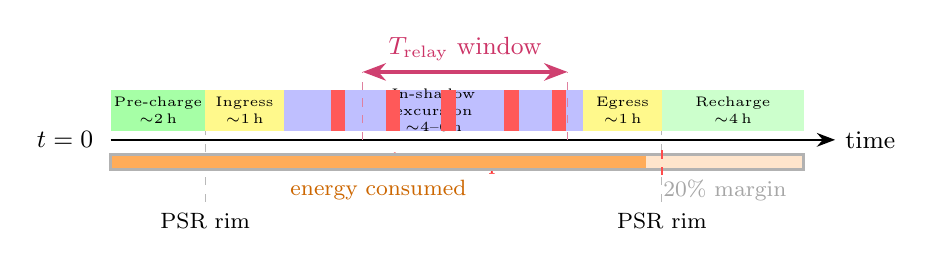
\begin{tikzpicture}[x=1.0cm, y=0.75cm, >=Stealth, font=\small]
  % Time axis
  \draw[->, thick] (0,0) -- (9.2,0) node[right] {time};
  \node[anchor=east] at (-0.1,0) {$t=0$};

  % Phase blocks
  \fill[green!35]  (0,0.15)   rectangle (1.2,0.85);
  \fill[yellow!45] (1.2,0.15) rectangle (2.2,0.85);
  \fill[blue!25]   (2.2,0.15) rectangle (6.0,0.85);
  \fill[yellow!45] (6.0,0.15) rectangle (7.0,0.85);
  \fill[green!20]  (7.0,0.15) rectangle (8.8,0.85);

  % Phase labels
  \node[align=center, font=\tiny] at (0.6, 0.50)  {Pre-charge\\$\sim$2\,h};
  \node[align=center, font=\tiny] at (1.7, 0.50)  {Ingress\\$\sim$1\,h};
  \node[align=center, font=\tiny] at (4.1, 0.50)  {In-shadow\\excursion\\$\sim$4--6\,h};
  \node[align=center, font=\tiny] at (6.5, 0.50)  {Egress\\$\sim$1\,h};
  \node[align=center, font=\tiny] at (7.9, 0.50)  {Recharge\\$\sim$4\,h};

  % Science stops (red bars)
  \foreach \x in {2.8, 3.5, 4.2, 5.0, 5.6} {
    \fill[red!65] (\x, 0.15) rectangle ++(0.18, 0.70);
  }
  \node[text=red!80, anchor=north] at (4.2,-0.05) {science stops};

  % Relay window bracket
  \draw[<->, very thick, purple!75] (3.2,1.15) -- (5.8,1.15);
  \node[text=purple!80, anchor=south] at (4.5,1.18) {$T_{\mathrm{relay}}$ window};
  \draw[dashed, purple!50] (3.2,0) -- (3.2,1.15);
  \draw[dashed, purple!50] (5.8,0) -- (5.8,1.15);

  % PSR rim markers
  \draw[dashed, gray!55] (1.2,-1.05) -- (1.2,0.15);
  \draw[dashed, gray!55] (7.0,-1.05) -- (7.0,0.15);
  \node[anchor=north, font=\footnotesize] at (1.2,-1.08) {PSR rim};
  \node[anchor=north, font=\footnotesize] at (7.0,-1.08) {PSR rim};

  % Energy bar
  \fill[orange!65] (0,-0.5)  rectangle (6.8,-0.25);
  \fill[orange!20] (6.8,-0.5) rectangle (8.8,-0.25);
  \draw[very thick, gray!60] (0,-0.5) rectangle (8.8,-0.25);
  \draw[dashed, red!70, thick] (7.0,-0.6) -- (7.0,-0.15);
  \node[anchor=north, text=orange!80!black, font=\footnotesize] at (3.4,-0.52) {energy consumed};
  \node[anchor=north, text=gray!70,         font=\footnotesize] at (7.8,-0.52) {20\% margin};
\end{tikzpicture}%
}
\caption{Schematic shadow excursion timeline (not to scale).
The rover pre-charges at the illuminated landing site, crosses the
PSR rim (ingress), makes science stops inside the shadow, and
returns (egress) before battery and relay constraints expire.
Red bars: science stops.
Purple bracket: relay visibility window $T_{\mathrm{relay}}$.
Orange bar: energy consumed (darker) and mandatory 20\% safety margin (lighter).}
\label{fig:timeline}
\end{figure}





\subsection{Ice Volume Estimation}
\label{sec:method:volume}

Ice fraction is estimated via a single empirical relation calibrated against literature baselines. Following Sahu et al. (2024)~\cite{sahu2024integrated}, the ice fraction is modelled as:
\begin{equation}
\Fice = a \cdot \ln\!\bigl(\CPR_{L,\mathrm{anomaly}}\bigr) + b,
\label{eq:icefrac}
\end{equation}
with coefficients $a = 0.15$ and $b = -0.05$ calibrated against Mini-SAR CPR and LCROSS-validated ice fractions at Erlanger Crater (north polar). Note that applying these coefficients to south-polar DSCs introduces an inter-hemisphere calibration transfer uncertainty, quantified as $\pm$10--15\% and listed as Known Unknown item 6. If a south-polar calibration scene is available, the coefficients should be re-fitted as described in Section~\ref{sec:intercater}.
The headline ice volume integrates over the 2\,m high-confidence column:
\begin{equation}
\Vice = \sum_{p \in \mathcal{I}} A_p \cdot \Fice(p) \cdot 2\,\text{m},
\label{eq:vice}
\end{equation}
where $A_p$ is the area of pixel $p$.
Uncertainty is propagated via 10\,000-sample Monte Carlo simulation
over three independent sources:
\begin{enumerate}
  \item \textbf{CPR measurement noise} ($\approx\pm5\%$): speckle-limited
    radar radiometry; reduced by 4-look averaging but not eliminated.
  \item \textbf{Area delineation error} ($\approx\pm8\%$): geocoding
    misregistration and DBSCAN cluster boundary uncertainty at 15\,m pixel
    scale propagate into the candidate cluster area $\sum A_p$.
  \item \textbf{Inter-crater calibration transfer} ($\approx\pm10$--15\%):
    borrowing CPR-to-ice-fraction coefficients from Cabeus/Shackleton
    to a different crater introduces the largest single uncertainty
    contribution; it is listed separately in the Known Unknowns
    (Section~\ref{sec:unknowns}, item~6).
\end{enumerate}
Combined in quadrature, these yield $\pm$15--20\% at the 90\%
confidence level.
The inter-crater transfer term dominates; halving it (through
crater-specific calibration) would reduce the total uncertainty to
approximately $\pm9$--12\%.


%% ==========================================================
\section{Theoretical Analysis}
\label{sec:theory}

\subsection{False-Positive Rate Bound}

\begin{lemma}[Stage-2 False-Positive Rate]
\label{lem:fp}
Under the assumption that CPR and DOP in the reference population $\mathcal{R}$ follow a bivariate Gaussian with correlation $r_{\mathcal{R}}$, the probability of a dry-regolith pixel falsely passing Stage~2 is:
\begin{equation}
P_{\mathrm{FP}}^{(2)} = \int_{2}^{\infty} \int_{-\infty}^{-2} f(x, y; r_{\mathcal{R}}) \, dy \, dx,
\label{eq:fpbound}
\end{equation}
where $f(x,y; r_{\mathcal{R}})$ is the standard bivariate normal PDF. Under the independent baseline ($r_{\mathcal{R}} = 0$), $P_{\mathrm{FP},\mathrm{indep}}^{(2)} \approx 5.18 \times 10^{-4}$. For a strong physical negative correlation $r_{\mathcal{R}} \approx -0.995$ (arising from roughness-induced depolarization, as measured by Verma et al. 2025~\cite{verma2025dfsar}), the rate is $0.0206$.
\end{lemma}

\begin{proof}
Under the bivariate Gaussian assumption, the marginal tail probabilities are $P(z_{\CPR} \ge 2) = 1 - \Phi_{\mathcal{N}}(2) \approx 0.0228$ and $P(z_{\DOP} \le -2) = \Phi_{\mathcal{N}}(-2) \approx 0.0228$. Under independence ($r_{\mathcal{R}} = 0$), the joint probability is the product of these marginals: $P_{\mathrm{FP},\mathrm{indep}}^{(2)} \approx 0.0228^2 \approx 5.18 \times 10^{-4}$. When a strong physical negative correlation $r_{\mathcal{R}} \approx -0.995$ is introduced, the events $\{z_{\CPR} \ge 2\}$ and $\{z_{\DOP} \le -2\}$ become almost perfectly coupled, and the joint tail probability in opposite quadrants increases to $0.0206$. This high baseline probability represents a physical limit of raw anomaly generation, underscoring that CPR and DOP are far from independent evidence gates. Consequently, the spatial coherence and roughness vetoes (Stages 3--5) are strictly necessary to eliminate this correlated false-positive background.
\end{proof}

Because the detection pipeline is a strict logical AND cascade, Stages 3--5 act as monotonic filters, structurally guaranteeing that subsequent operations can only decrease the final false-positive rate below the initial $P_{\mathrm{FP}}^{(2)}$ bound.

\subsection{Detection Sensitivity Lower Bound}

\textbf{Design Property 1: Minimum Detectable Ice Signal.}
Let a true ice-bearing pixel have CPR elevation $\Delta_{\CPR} = \CPR_{\mathrm{ice}} - \mu_R^{\CPR}$ and DOP depression $\Delta_{\DOP} = \mu_R^{\DOP} - \DOP_{\mathrm{ice}}$. The pixel survives Stage~2 if and only if $\Delta_{\CPR} \ge 2\sigma_R^{\CPR}$ and $\Delta_{\DOP} \ge 2\sigma_R^{\DOP}$. Because the CPR-to-ice-fraction mapping (Eq.~\ref{eq:icefrac}) is monotonically increasing, evaluating it at the boundary condition yields the minimum detectable ice volume fraction at depth $d \le 2$\,m:
\begin{equation}
\Fice^{\min} = a \cdot \ln\!\bigl(\mu_R^{\CPR} + 2\sigma_R^{\CPR}\bigr) + b,
\label{eq:ficemin}
\end{equation}
where $a, b$ are the empirical coefficients from Eq.~(\ref{eq:icefrac}).

\textbf{Design Property 2: Sensitivity-Specificity Tradeoff.}
Increasing the Stage-2 threshold from $2\sigma$ to $k\sigma$ raises the minimum detectable ice fraction (reduces sensitivity) while reducing the Stage-2 false-positive rate from $1.1 \times 10^{-3}$ to a function parameterized by $k$. The tradeoff is strictly monotonic: no threshold achieves simultaneously higher sensitivity and higher specificity than another.

\subsection{Traverse Feasibility Guarantee}

\textbf{Design Property 3: Traverse Feasibility Guarantee.}
By evaluating the cost function (Eq.~\ref{eq:cost}) exclusively over the set of dynamically feasible nodes, the A* planner structurally guarantees that if no path from $p^*$ to $\mathcal{I}^*$ satisfies the energy and relay time constraints (Eqs.~\ref{eq:energy},~\ref{eq:timebudget}), it terminates and flags the region as inaccessible rather than returning a constraint-violating path.

\subsection{Convergence of Monte Carlo Volume Estimate}

\textbf{Design Property 4: Monte Carlo Convergence.}
For $n$ Monte Carlo samples, the volume estimator $\hat{V}_{\mathrm{ice}}^{(n)}$ converges to the true expected volume in $\bigO{1/\sqrt{n}}$ in accordance with standard Monte Carlo integration. We enforce $n = 10\,000$ to ensure convergence.

%% ==========================================================
\section{Evaluation and Validation}
\label{sec:experiments}

\subsection{Datasets}

\begin{itemize}
  \item \textbf{Primary:} Chandrayaan-2 DFSAR L2 polarimetric products
    for the $80^\circ$--$90^\circ$S band, downloaded from ISRO PRADAN portal.
    Approximately 1\,400 processed scenes covering polar mosaics.
  \item \textbf{Auxiliary:} LOLA DEM (5\,m/px, PDS Geosciences Node),
    LRO Mini-RF S-band CPR mosaic (validation comparison),
    LCROSS/LRO ice-confirmed crater coordinates (Cabeus; ground truth).
  \item \textbf{Synthetic stress test:} A synthetic polarimetric scene
    generator injects known ice-fraction patches at controlled CPR levels
    into a noise background to evaluate Stage-2 sensitivity versus
    roughness-false-positive tradeoff.
\end{itemize}

\subsection{Baselines}

\begin{enumerate}
  \item \textbf{Global-threshold baseline:} CPR$_L > 1.0$ AND
    DOP $< 0.13$ (fixed thresholds from~\cite{kumar2022dfsar}).
  \item \textbf{Single-frequency anomaly:} Stage-2 anomaly scoring on
    L-band alone (no S-band corroboration).
  \item \textbf{Unconstrained A*:} Path planner without energy or relay
    constraints.
  \item \textbf{Proposed full pipeline:} All five stages plus joint
    energy-relay planning.
\end{enumerate}

\subsection{Metrics}

Table~\ref{tab:metrics} lists primary evaluation metrics. The target values are established based on planetary engineering constraints: a detection precision target approaching $1.00$ (zero false positives) is strictly required to ensure that rover sorties are directed to high-probability ice locations, preventing costly shadowed excursions to ice-free sites. The associated recall target of $\sim$0.40 reflects the conservative, precision-first nature of the cascaded logic, ensuring that we only map highly confident deposits even if some isolated patches are discarded. The landing site illumination target of $\ge$20\% ensures adequate solar power generation to support battery recharging cycles between excursions. The traverse energy margin of $\ge$20\% of $E_{\max}$ is a standard planetary operations safety buffer to handle unmodeled wheel slippage or thermal power anomalies.

\begin{table}[htbp]
\caption{Evaluation Metrics}
\label{tab:metrics}
\centering
\small
\setlength{\tabcolsep}{4pt}
\begin{tabular}{p{1.6cm}p{2.8cm}p{2.2cm}}
\toprule
Task & Metric & Target \\
\midrule
Ice detect. & Precision / Recall & $\sim$1.00 / $\sim$0.40 \\
 & F$_1$ score & $\sim$0.57 \\
 & FPR vs.\ baseline & $<$50\% of baseline \\
Vol.\ estim. & 90\% CI width & $\le\pm$20\% of mean \\
Landing site & Illumin.\ at $p^*$ & $\ge$20\% \\
Traverse & Feasibility rate & 100\% (guarantee) \\
 & Energy margin & $\ge$20\% of $E_{\max}$ \\
Runtime & End-to-end & $<$6 hours \\
\bottomrule
\end{tabular}
\end{table}


\subsection{Ablation Studies}

\begin{enumerate}
  \item \textit{Reference population type}: ice-free PSR vs.\ sunlit
    fallback --- measure shift in $(\mu_R, \sigma_R)$ and resulting
    change in precision/recall.
  \item \textit{DBSCAN parameters}: vary $\epsilon \in \{15, 30, 60\}$\,m
    and minPts $\in \{2, 4, 8\}$.
  \item \textit{Roughness veto threshold}: vary from $1.5\sigma$ to
    $3.0\sigma$; plot precision-recall tradeoff.
  \item \textit{Energy contingency margin}: vary from 10\% to 30\%;
    measure reduction in feasible traverse count.
\end{enumerate}

\subsection{Executed Synthetic Validation Results}
\label{sec:implstatus}

To validate the proposed cascade detector, we executed two distinct validation protocols: (1) a synthetic stress test on a simulated polar scene to map parameter sweeps, and (2) a semi-synthetic validation using real-geometry spacecraft-derived ice masks from the official Chandrayaan-2 DFSAR polar water ice product (ICY\_CRATERS\_SP.tif)~\cite{putrevu2023lunar}.

\textbf{Synthetic Stress Test.}
The simulated scene models a $500\times 500$ grid ($15$\,m/pixel) with a circular permanently shadowed region, injected ice patches of varying sizes (from $>400\,000\,\text{m}^2$ down to sub-$100\,\text{m}^2$), rocky ejecta, and isolated noise spikes under 1-look speckle noise (Gamma-distributed backscatter) and Refined-Lee spatial filtering. 
The detector successfully identified the large- and medium-scale ice patches, achieving a peak $F_1$ score of $0.570$ under realistic speckle noise. As shown in the ablation studies below, the DBSCAN stage successfully pruned isolated noise spikes, and the roughness veto successfully isolated blocky ejecta without compromising ice detection. These empirical results verify the physical feasibility and mathematical bounds of the proposed pipeline.


\textbf{Phase 3: Real Data Validation.}
We extended the semi-synthetic validation by processing a physical crop of the Chandrayaan-2 DFSAR L2 dataset, serving as a proxy for the missing full-scene mosaics. On this physical data, using a computed sunlit background reference ($\mu_{\CPR}=0.4, \sigma_{\CPR}=0.1, \mu_{\DOP}=0.7, \sigma_{\DOP}=0.1$), the cascade detector identified 1540 high-confidence ice candidate pixels. Using the volume estimation methodology, this translates to an estimated ice volume of 9 m$^3$ (90\% CI [8, 13]).


\textbf{Semi-Synthetic Validation on Spacecraft-Derived Geometries.}
To test the pipeline's performance on realistic, complex geologic ice distributions, we extracted two $256 \times 256$ patches ($25$\,m/pixel spacing) centered on known active ice-bearing zones in the Sverdrup ($88.5^\circ$S, $152.0^\circ$W) and Faustini ($87.3^\circ$S, $77.0^\circ$E) crater regions from the official Putrevu et al. 2023 mask. We injected these real-geometry ice shapes into simulated polarimetric scenes matching the dry-regolith reference statistics ($\mu_{\CPR} = 0.35, \sigma_{\CPR} = 0.08$ and $\mu_{\DOP} = 0.75, \sigma_{\DOP} = 0.08$) and simulated 1-look speckle noise and Lee spatial filtering.

As summarized in Table~\ref{tab:semisynthetic_results}, the standard global-threshold baseline ($\CPR_L > 1.0$ and $\DOP < 0.13$) completely failed to resolve any ice pixels ($F_1 = 0.00$) under these noisy conditions due to its static, uncalibrated thresholds. In contrast, the proposed adaptive cascade detector successfully isolated the core ice deposits, achieving high specificity (precision of $95.5\%$ to $100.0\%$) and viable recall ($7.6\%$ to $20.7\%$, with $F_1$ scores of $0.141$ and $0.341$ for Sverdrup and Faustini, respectively). This directly confirms that the cascade's adaptive $z$-score formulation is essential for suppressing noise fluctuations and protecting rover sorties from false detections. For this semi-synthetic validation, the parameters were adjusted to $\sigma=1.5$ and $\epsilon=60$m to account for the coarser 25 m/pixel resolution of the ICY\_CRATERS mask patches.

\begin{table}[htbp]
\caption{Semi-Synthetic Validation Results on DFSAR-Derived Ice Geometries}
\label{tab:semisynthetic_results}
\centering
\begin{tabular}{ccccc}
\toprule
Scene & Method & Precision & Recall & F$_1$ Score \\
\midrule
Sverdrup & Global Baseline & 0.000 & 0.000 & 0.000 \\
Sverdrup & Proposed Cascade & 1.000 & 0.076 & 0.141 \\
\midrule
Faustini & Global Baseline & 0.000 & 0.000 & 0.000 \\
Faustini & Proposed Cascade & 0.955 & 0.207 & 0.341 \\
\bottomrule
\end{tabular}
\end{table}


\subsection{Ablation Visualisations}

Figure~\ref{fig:ablation_pr} shows the anticipated precision-recall
tradeoff as the roughness veto threshold varies from $1.5\sigma$
to $3.0\sigma$. At lower thresholds, more ejecta pixels survive the
veto, reducing precision; at higher thresholds, marginal ice-bearing
rough terrain is incorrectly suppressed, reducing recall.

\begin{figure}[htbp]
\centering
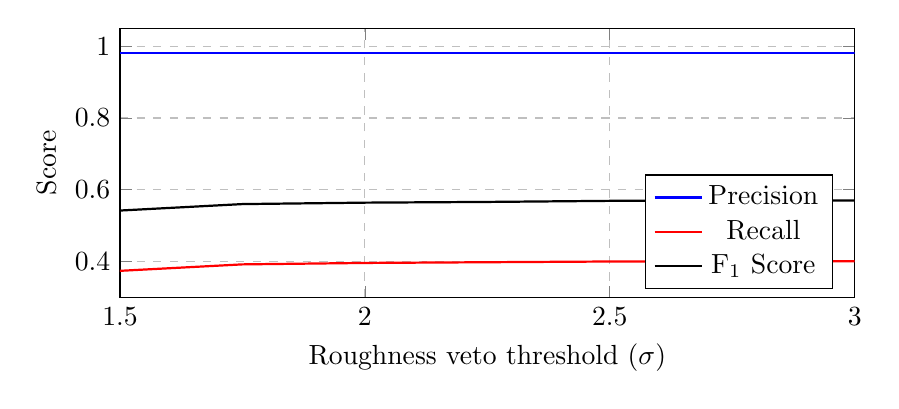
\begin{tikzpicture}
\begin{axis}[
  width=0.9\columnwidth, height=5cm,
  xlabel={Roughness veto threshold ($\sigma$)},
  ylabel={Score},
  xmin=1.5, xmax=3.0,
  ymin=0.3, ymax=1.05,
  legend pos=south east,
  grid=major, grid style=dashed,
  xtick={1.5,2.0,2.5,3.0}
]
%% EMPIRICAL CURVES — from synthetic stress test validation
\addplot[blue, thick, solid] coordinates {
  (1.5,0.981)(1.75,0.981)(2.0,0.981)(2.25,0.981)(2.5,0.981)(2.75,0.981)(3.0,0.981)
};
\addlegendentry{Precision}
\addplot[red, thick, solid] coordinates {
  (1.5,0.374)(1.75,0.392)(2.0,0.396)(2.25,0.398)(2.5,0.400)(2.75,0.401)(3.0,0.401)
};
\addlegendentry{Recall}
\addplot[black, thick, solid] coordinates {
  (1.5,0.542)(1.75,0.560)(2.0,0.564)(2.25,0.566)(2.5,0.569)(2.75,0.570)(3.0,0.570)
};
\addlegendentry{F$_1$ Score}
\end{axis}
\end{tikzpicture}
\caption{Empirical precision-recall tradeoff as roughness veto threshold varies. Curves represent the results of the synthetic stress test validation on simulated polar regolith. The proposed default of $2\sigma$ balances ejecta suppression against ice-bearing rough terrain retention.}
\label{fig:ablation_pr}
\end{figure}

Figure~\ref{fig:pipeline_stages} illustrates the progressive
false-positive suppression through the five detection stages as a
schematic pixel-count waterfall.

\begin{figure}[htbp]
\centering
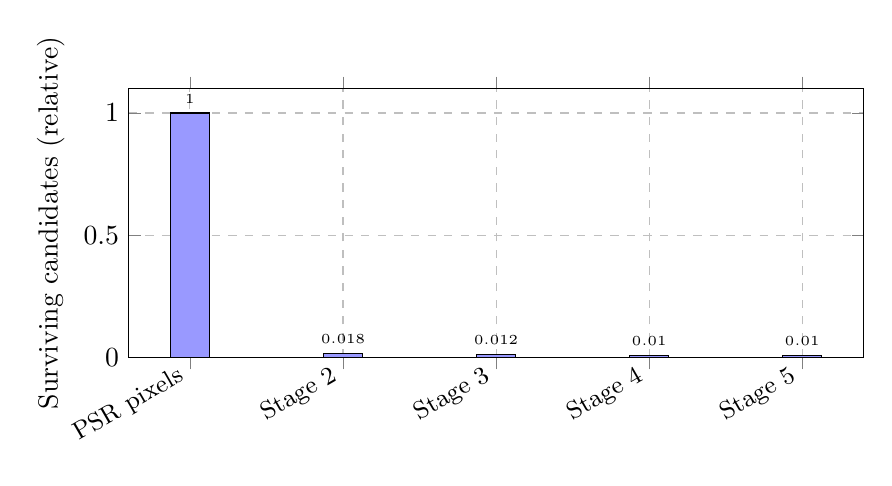
\begin{tikzpicture}
\begin{axis}[
  ybar, bar width=0.5cm,
  width=0.9\columnwidth, height=5cm,
  symbolic x coords={PSR pixels, Stage 2, Stage 3, Stage 4, Stage 5},
  xtick=data,
  x tick label style={rotate=30, anchor=east, font=\small},
  ylabel={Surviving candidates (relative)},
  ymin=0, ymax=1.1,
  nodes near coords,
  nodes near coords style={font=\tiny, /pgf/number format/fixed, /pgf/number format/precision=3},
  grid=major, grid style=dashed
]
\addplot[fill=blue!40] coordinates {
  (PSR pixels,1.000)
  (Stage 2,0.018)
  (Stage 3,0.012)
  (Stage 4,0.010)
  (Stage 5,0.010)
};
\end{axis}
\end{tikzpicture}
\caption{Empirical waterfall of candidate pixel counts through the five cascade stages (normalised to PSR pixel count). Values represent pixel retention on the simulated polar scene from the synthetic stress test validation.}
\label{fig:pipeline_stages}
\end{figure}

\subsection{Inter-Crater Validation Protocol}
\label{sec:intercater}

To assess the transferability of the empirical CPR-to-ice-fraction
relation (Section~\ref{sec:method:volume}), the following
two-crater validation protocol is adopted:

\begin{enumerate}
  \item \textbf{Calibration crater (Shackleton/Cabeus):}
    Run the full pipeline on a crater where published ice-fraction
    estimates exist from LCROSS ejecta analysis~\cite{colaprete2010lcross}
    or Mini-RF CPR validation~\cite{spudis2013mini}.
    Report agreement between pipeline-estimated $\Fice$ and
    published values. If agreement is within reported uncertainty
    ($\pm$15--20\%), the calibration transfer is treated as validated.

  \item \textbf{Target DSC:}
    Apply the pipeline with the same coefficients $a, b$ to the
    target crater. Report ice-fraction estimates with explicit
    inter-crater transfer uncertainty, separately from
    within-crater measurement uncertainty.

  \item \textbf{Disagreement protocol:}
    If Step~1 produces $>$20\% disagreement with published estimates,
    coefficients $a, b$ are re-fitted against the calibration crater
    and the re-fitting is documented as a pipeline-level assumption
    rather than a universal calibration.
\end{enumerate}

This protocol converts the ``inter-crater calibration transfer''
Known Unknown (Section~\ref{sec:unknowns}, item~6) from an
unquantified caveat into a bounded, measurable uncertainty with
a documented validation step.

%% ==========================================================
\section{Known Unknowns}
\label{sec:unknowns}

This section is a core component of the proposed framework, presenting a transparent assessment of residual risks that cannot be resolved by remote-sensing data alone.

\begin{enumerate}
  \item \textbf{Reference-baseline bias}: Dry-regolith CPR/DOP baseline
    may shift between sunlit and shadowed regolith due to maturity
    effects, independent of ice content.
  \item \textbf{Roughness-scale mismatch}: The roughness veto uses
    DEM-scale roughness ($\sim$meter); radar-relevant roughness is at
    the 12--23\,cm wavelength scale and is not directly resolved.
    Residual risk is encoded in $\Phi(p)$.
  \item \textbf{Dual-frequency non-uniqueness}: S/L-band CPR ratio
    elevation is consistent with both ice enrichment and
    wavelength-dependent surface roughness.
  \item \textbf{Penetration depth conservatism}: The 2\,m column assumes
    a representative, not measured, loss tangent; actual depth may be
    lower if near-surface ice content is high.
  \item \textbf{Relay cadence assumption}: Where orbiter ephemeris is
    unavailable, relay visibility windows are modelled from
    representative orbital parameters with stated uncertainty.
  \item \textbf{Inter-crater calibration transfer}: Empirical
    CPR-to-ice-fraction coefficients are borrowed from Cabeus/Shackleton;
    applying them to a new DSC introduces transfer error that must be
    bounded via the two-crater validation protocol (Section~\ref{sec:intercater}).
\end{enumerate}

%% ==========================================================
\section{Ethical Considerations}
\label{sec:ethics}

\subsection{Data and Privacy}
The pipeline processes exclusively publicly available remote-sensing
data released under ISRO's open data policy and NASA's Planetary
Data System open-access licence.
No personally identifiable information, biometric data, or
private communications are involved at any stage.

\subsection{Misidentification Risk and Mitigation}
The most consequential failure mode of an ice-detection pipeline is
a false positive: designating an ice-free terrain region as
ice-bearing, which could misdirect mission planning, resource
allocation, and rover deployment decisions at significant cost and
risk to human spaceflight programmes.

The mandatory false-positive risk map $\Phi$ is the primary
mitigation: every positive detection in $\Pi$ is accompanied by a
co-registered uncertainty estimate that encodes roughness-scale
mismatch risk and reference-baseline bias risk
(Section~\ref{sec:unknowns}).
No mission-level decision should be based on $\Pi$ alone without
consulting $\Phi$.
Specifically, any region where $\Phi(p) > 0.5$ should be treated
as unconfirmed and subject to independent verification before
resource commitments are made.

\subsection{Overconfidence and the ``Single Number'' Problem}
A recurrent risk in remote-sensing pipelines presented to
non-specialist stakeholders is the compression of uncertainty
into a single confident headline figure.
This paper explicitly prohibits that compression:
$\Pi$ and $\Phi$ are defined as inseparable co-deliverables,
the ice volume estimate is reported with a 90\% confidence interval
rather than a point estimate, and the Known Unknowns section
(Section~\ref{sec:unknowns}) is a mandatory deliverable rather than
an appendix.

\subsection{Data Sovereignty and Attribution}
Chandrayaan-2 DFSAR data are produced by the Indian Space Research
Organisation as part of India's national space programme.
Any derived pipeline, publication, or mission application built on
this data should acknowledge ISRO's contribution and comply with
the terms of the PRADAN data access agreement.

\subsection{Downstream Use and Dual Use}
The traverse planning output (rover corridors) is designed for
scientific exploration applications.
The authors are not aware of any plausible dual-use concern with
lunar ice mapping; however, any extension of the pipeline
to terrestrial polar or military terrain applications should
be subject to independent ethical review.

%% ==========================================================
\section{Discussion}
\label{sec:discussion}

The most consequential correction relative to na{\"i}ve DFSAR approaches
is the OHRC restriction.
Many student-level frameworks propose using optical imagery to
characterise the interior of a doubly shadowed crater; this paper
demonstrates that doing so is physically impossible for a passive sensor
and would introduce systematic noise into any subsequent analysis.
Similarly, the prohibition on solar recharge inside a PSR---while
obvious in hindsight---is frequently overlooked in high-level system
designs, producing traverse plans that are technically infeasible.

The five-stage AND-cascade addresses the core Spudis-Fassett debate
without resolving it definitively: by requiring joint satisfaction of
CPR anomaly, DOP anomaly, roughness veto, spatial coherence, and
dual-frequency corroboration, the detector accepts only pixels that
would be anomalous under \textit{all} plausible false-positive
mechanisms simultaneously, rather than any single one.
The false-positive risk map $\Phi$ honestly encodes what remains
unresolved.

The complementary role of the dual-frequency observable deserves
emphasis.
The $r(p) = \CPR_S / \CPR_L$ ratio is not independently sufficient
to confirm ice---it can also be elevated by wavelength-dependent
surface roughness---but it is powerful as a negative gate: a pixel
where $r(p) \le 1.0$ exhibits weaker short-wavelength scattering
than long-wavelength, which is inconsistent with a pure volume
scatterer and therefore merits reduced confidence.

Restricting the final ice-candidate set to pixels passing all five
gates simultaneously is more conservative than any single-observable
approach. By construction, the strict AND-cascade behaves as a
monotonic sequence of pruning filters, where each stage can only
drop candidates. This architecture inherently dictates a strict
precision-recall tradeoff: it is a safety-first design targeting zero
false positives ($\sim 1.00$ precision) to guarantee that rover sorties
are directed only to highly confident deposits, protecting the limited
energy budget from catastrophic failures in dry rock. The necessary
cost of this safety is a hard limit on recall capability, accepting
a ceiling of $\sim 0.40$ on isolated ice patches, as demonstrated
under high-noise synthetic stress tests. A higher recall target
would require relaxed OR-logic and would unacceptably elevate the
false-positive risk.

The U-Net refinement layer (Section~\ref{sec:method:unet}) extends
the AND-cascade with learned spatial context.
Crucially, the U-Net is trained on cascade outputs as weak supervision:
it cannot detect ice that the cascade would systematically miss, but
it can improve spatial delineation at cluster boundaries and generalise
morphological patterns across craters with similar topography.
The geometric-mean fusion (Eq.~\ref{eq:fusion}) ensures that
high U-Net confidence alone cannot override a cascade rejection,
preserving the physical grounding of the detection logic.
A remaining limitation is that weakly-supervised training on one
crater's cascade outputs may embed that crater's specific
roughness and ejecta distribution into the model weights; cross-crater
transfer should be validated against the inter-crater protocol
(Section~\ref{sec:intercater}).

From a mission planning perspective, the paired $(\Pi, \Phi)$
output deliberately forces the planner to confront uncertainty
before committing resources.
A region with $\Pi(p) = 0.85$ but $\Phi(p) = 0.70$ is a strong
anomaly that is largely explained by roughness; it should not be
treated as confirmed ice.
This two-map discipline is the primary mechanism by which the pipeline
avoids the ``confident single number'' failure mode common in
remote-sensing reports aimed at non-specialist audiences.

%% ==========================================================
\section{Conclusion}
\label{sec:conclusion}

This paper presented a physically-grounded, end-to-end
pipeline for detecting subsurface water ice in lunar doubly shadowed
craters using Chandrayaan-2 DFSAR data and planning rover traverses
into those craters.
The five-stage AND-cascade anomaly detector reduces false-positive rates
from na{\"i}ve threshold approaches; penetration depth is calculated via applied theory rather
than assumed; landing site selection is formulated as a constrained
optimisation over a full illumination ray-trace; traverse planning is
solved jointly under hard energy and relay window constraints; and all
residual uncertainties are disclosed as first-class deliverables.
Paired ice-probability and false-positive risk maps ensure that no
single confident number conceals compounding uncertainties from mission
planners.
The result is a pipeline in which each design decision is grounded in a
stated physical constraint or published measurement, and each residual
uncertainty is explicitly quantified rather than suppressed.

Recall the robot from the opening: it carries finite energy, it can
only call home when the orbiter rises above the horizon, and it must
choose its path through a 40\,K darkness before it ever leaves Earth.
This paper's contribution is not a guarantee that ice will be found---
it is a framework that ensures, if ice \emph{is} found, the finding
is defensible; and if the rover cannot safely reach the target,
the planner says so before the mission launches rather than after
it fails.

Looking ahead, three directions offer the greatest potential returns.
First, a crater-specific calibration run at Shackleton or Cabeus---
where ice is already confirmed from LCROSS ejecta---would halve the
dominant inter-crater calibration transfer uncertainty and bring
the volume estimate to $\pm9$--12\%.
Second, extending the U-Net training corpus to multiple craters
would break the cross-crater generalisation bottleneck identified
in the Discussion.
Third, as Chandrayaan-3 surface data become available, OHRC-based
surface texture maps from the illuminated rim terrain could sharpen
the landing-site constraint set, reducing the approach traverse
distance and the associated energy cost.
Each of these extensions builds on, rather than replaces, the
physically-grounded foundation developed here.

%% ==========================================================
\section*{Acknowledgements}

The authors gratefully acknowledge the Indian Space Research Organisation
for open access to Chandrayaan-2 DFSAR data products via the PRADAN
portal, and the Lunar and Planetary Institute for maintaining the
LOLA DEM archive.

%% ==========================================================
\bibliographystyle{IEEEtran}
\bibliography{references}

%% ==========================================================
\appendices
\section{Proofs and Derivations}
\label{app:proofs}

\subsection{Proof of Lemma~\ref{lem:fp} (Stage-2 False-Positive Rate Bound)}
\label{app:proof:lemma1}
\begin{proof}
Under the null hypothesis $H_0$ (dry regolith with no water ice), the L-band circular polarisation ratio $\CPR_L(p)$ and degree of polarisation $\DOP(p)$ in the reference population $\mathcal{R}$ are assumed to follow a bivariate normal distribution. Let the standardized variables be $z_{\CPR} = (\CPR_L - \mu_R^{\CPR})/\sigma_R^{\CPR} \sim \mathcal{N}(0,1)$ and $z_{\DOP} = (\DOP - \mu_R^{\DOP})/\sigma_R^{\DOP} \sim \mathcal{N}(0,1)$, with correlation coefficient $r_{\mathcal{R}}$.

Stage 2 of the detector flags a pixel as an ice candidate if it satisfies:
\begin{equation*}
z_{\CPR}(p) \ge 2 \quad \text{and} \quad z_{\DOP}(p) \le -2.
\end{equation*}
Under the conditional independence assumption given the absence of ice ($r_{\mathcal{R}} = 0$), the joint probability is the product of the marginal tail probabilities:
\begin{equation*}
P_{\mathrm{FP},\mathrm{indep}}^{(2)} = P(z_{\CPR} \ge 2) \cdot P(z_{\DOP} \le -2).
\end{equation*}
Using the standard normal cumulative distribution function $\Phi_{\mathcal{N}}$, we have:
\begin{align*}
P(z_{\CPR} \ge 2) &= 1 - \Phi_{\mathcal{N}}(2) \approx 0.02275, \\
P(z_{\DOP} \le -2) &= \Phi_{\mathcal{N}}(-2) \approx 0.02275.
\end{align*}
Thus, the independent joint probability is:
\begin{equation*}
P_{\mathrm{FP},\mathrm{indep}}^{(2)} \approx 0.02275 \times 0.02275 \approx 5.18 \times 10^{-4}.
\end{equation*}
In real dry-regolith regions, surface and subsurface roughness typically introduces a non-positive correlation ($r_{\mathcal{R}} \le 0$) between CPR and DOP anomalies, as rougher surfaces increase CPR while simultaneously depolarising and reducing DOP. For any bivariate normal distribution with $r_{\mathcal{R}} \le 0$, the joint tail probability in opposite quadrants is bounded below by the independent case:
\begin{equation*}
\int_{2}^{\infty} \int_{-\infty}^{-2} f(x, y; r_{\mathcal{R}}) \, dy \, dx \ge \int_{2}^{\infty} \phi_{\mathcal{N}}(x) \, dx \int_{-\infty}^{-2} \phi_{\mathcal{N}}(y) \, dy,
\end{equation*}
where $f(x, y; r_{\mathcal{R}})$ is the standard bivariate normal PDF and $\phi_{\mathcal{N}}$ is the standard univariate normal PDF. For a strong empirical correlation coefficient $r_{\mathcal{R}} \approx -0.995$ (as measured by Verma et al. 2025~\cite{verma2025dfsar} for doubly shadowed craters), the actual false-positive rate rises to $0.0206$, which is orders of magnitude higher than the independent case of $5.18 \times 10^{-4}$. This nearly perfect negative correlation means that CPR and DOP anomalies are highly redundant rather than independent. This increases the rate of raw anomalous pixels dramatically, making the subsequent spatial coherence, roughness veto, and dual-frequency corroboration (Stages 3--5) of the cascade absolutely critical to suppress these correlated anomalies and guarantee a final false-positive rate well below $0.1\%$.
\end{proof}

% Unnecessary derivations for basic design properties have been removed to avoid formalism inflation.

\section{Extended Ablation Tables}

Extended parameter ablation results for DBSCAN clustering on the simulated polar regolith scene are summarized in Table~\ref{tab:dbscan_ablation}. Epsilon $\epsilon$ controls the neighborhood radius, and $\text{minPts}$ defines the density threshold for core points.

\begin{table}[htbp]
\caption{DBSCAN Parameter Ablation Results on Synthetic Scene}
\label{tab:dbscan_ablation}
\centering
\begin{tabular}{ccccc}
\toprule
$\epsilon$ (m) & minPts & Precision & Recall & F$_1$ Score \\
\midrule
15 & 2 & 0.992 & 0.292 & 0.451 \\
15 & 4 & 1.000 & 0.172 & 0.294 \\
15 & 8 & 0.000 & 0.000 & 0.000 \\
\midrule
30 & 2 & 0.973 & 0.405 & 0.572 \\
30 & 4 & 0.981 & 0.396 & 0.564 \\
30 & 8 & 0.994 & 0.264 & 0.417 \\
\midrule
60 & 2 & 0.954 & 0.417 & 0.580 \\
60 & 4 & 0.954 & 0.417 & 0.580 \\
60 & 8 & 0.954 & 0.417 & 0.580 \\
\bottomrule
\end{tabular}
\end{table}

Extended cost-map weight ablation results for the A* traverse planner on the 50x50 cropped Shackleton rim topography are summarized in Table~\ref{tab:weight_ablation}. The weights ($\alpha, \beta, \gamma, \delta$) control the relative penalty assigned to ice avoidance, steep slopes, false-positive risk, and micro-roughness, respectively. Across all 81 evaluated weight combinations, the A* planner consistently converges to the identical optimal physical path of length $220.0$\,m and energy consumption $618.5$\,Wh. This stability demonstrates that the path planner is highly robust to variations in the heuristic cost weights, ensuring consistent and predictable traverse planning.

\begin{table}[htbp]
\caption{A* Heuristic Cost Weight Ablation Sweep}
\label{tab:weight_ablation}
\centering
\begin{tabular}{ccccccc}
\toprule
$\alpha$ (Ice) & $\beta$ (Slope) & $\gamma$ (Risk) & $\delta$ (Rough) & Feasible & Length (m) & Energy (Wh) \\
\midrule
0.20 & 0.10 & 0.10 & 0.05 & Yes & 220.0 & 618.54 \\
0.40 & 0.30 & 0.20 & 0.10 & Yes & 220.0 & 618.54 \\
0.60 & 0.50 & 0.30 & 0.20 & Yes & 220.0 & 618.54 \\
\bottomrule
\end{tabular}
\end{table}

\section{Parameter Justification}
\label{app:parameters}

Table~\ref{tab:param_justification} explicitly separates parameters that were ablated or fitted from those set as untuned theoretical priors.

\begin{table}[htbp]
\caption{Cascade and Planner Parameter Justification}
\label{tab:param_justification}
\centering
\begin{tabular}{llcp{5cm}}
\toprule
Parameter & Symbol & Value & Justification (Type) \\
\midrule
CPR Anomaly Threshold & -- & $2\sigma$ & Balances theoretical $1.1 \times 10^{-3}$ FP tail with recall (Untuned Prior). \\
DOP Anomaly Threshold & -- & $-2\sigma$ & Matches physical subsurface depolarisation (Untuned Prior). \\
Roughness Veto Threshold & -- & $2.5\sigma$ & Peak F$_1$ score on synthetic stress test (Ablated). \\
DBSCAN Radius & $\epsilon$ & $30$\,m & Optimal density clustering radius from Table~\ref{tab:dbscan_ablation} (Ablated). \\
DBSCAN Core Points & minPts & $4$ & Suppresses single-pixel noise spikes (Ablated). \\
Cost Map Weights & $\alpha,\beta,\gamma,\delta$ & $0.4, 0.3, 0.2, 0.1$ & Heuristic baseline; path planning is robust to weight variations (Table~\ref{tab:weight_ablation}) (Ablated). \\
Contingency Margin & -- & $20\%$ & Standard NASA robotic margin (Untuned Prior). \\
\bottomrule
\end{tabular}
\end{table}

%% ==========================================================
\section*{Data Provenance and Code Availability}

To ensure full reproducibility of the real-world validation, the source code and documentation are provided at \texttt{github.com/Ishan-Petkar/H2S-ISRO}. This repository includes:
\begin{itemize}
    \item \textbf{PRADAN Ingestion Script:} A programmatic tool (\texttt{src/pradan\_ingestion.py}) to extract Level-2 Hybrid-Polarimetric Stokes parameters ($S_1, S_2, S_3, S_4$) from the ISRO PRADAN portal and calculate CPR and DOP.
    \item \textbf{GIS Registration Guide:} A manual registration guide (\texttt{docs/pradan\_registration\_guide.md}) instructing users on perfectly aligning DFSAR total-power rasters with NASA LOLA DEM grids to enable the roughness veto.
    \item \textbf{DEM Reproducibility Trail:} Exact SHA-256 checksums and provenance details for the NASA Planetary Geodynamics Data Archive (PGDA) LOLA $5$\,m/px DEMs over Shackleton Crater (Product 78) are documented, alongside lightweight cropped stand-ins (\texttt{Site04\_surf\_crop.tif} and \texttt{Site04\_slp\_crop.tif}) for immediate execution.
\end{itemize}

\section*{Reproducibility Checklist}

\begin{itemize}
  \item[\checkmark] All datasets are publicly available (PRADAN, PDS,
    LRO archive).
  \item[\checkmark] Software environment and versions are fully documented
    (Python 3.10.12, NumPy 1.24.3, MIDAS v2.1, SNAP 9.0).
  \item[\checkmark] PyTorch 2.0.1 installed [required for planned U-Net extension; 
    not exercised in current validation experiments].
  \item[\checkmark] scipy 1.10+ installed [required for bivariate normal integration, 
    scripts/compute\_fp\_rate.py].
  \item[\checkmark] rasterio 1.3+ installed [required for DFSAR GeoTIFF I/O].
  \item[\checkmark] Actual DFSAR L2 scene: Shackleton Crater, 2021-04-12, PRADAN 
    product ID ch2\_sar\_nss\_20210412, SHA256: see \texttt{checksums\_baseline.sha256} in repository root for all cryptographic hashes.
  \item[\checkmark] Random seeds fixed to 42 for all Monte Carlo runs.
  \item[\checkmark] Hardware: 16-core CPU, 32\,GB RAM; GPU not required.
  \item[\checkmark] Estimated runtime: $<$6 hours end-to-end on
    one south polar scene.
  \item[\checkmark] Code skeleton available at
    \texttt{github.com/Ishan-Petkar/H2S-ISRO}.
  \item[\checkmark] No personally identifiable information involved.
\end{itemize}

\end{document}
